% !Mode:: "TeX:UTF-8"
\chapter{积分论}

\begin{introduction}
	\item 非负可测简单函数的Lebesgue积分
	\item 非负可测函数的Lebesgue积分 (Levi、Fatou)
	\item 一般可测函数的Lebesgue积分
	\item Lebesgue控制收敛定理
	\item Riemann积分与Lebesgue积分的关系
	\item 重积分与累次积分的关系
\end{introduction}

Lebesgue积分是在Lebesgue测度论的基础上建立起来的. 
这一理论可以统一处理函数有界与无界的情形, 
而且函数也可以定义在更一般的点集(不一定是闭区间$[a,b]$上). 
特别的, 它提供了比Riemann积分更加广泛而有效的收敛定理. 

定义Lebesgue积分有着各种不同的等价方法, 
我们在这里所采用的是, 首先定义非负可测简单函数的积分, 
再注意到可测简单函数与非负可测函数的关系, 就可以给出后者的积分定义, 
最后通过表示 式 $f(x)=f^{+}(x)-f^{-}(x)$, 也就有了一般可测函数的积分定义. 
这种建立积分的途径也适用于一般测度空间上的积分.

\section{Lebesgue积分理论}
\subsection{非负可测简单函数的Lebesgue积分}

\begin{definition}[非负可测简单函数的积分]
	设$\varphi(x)$为$E \subset \R^n$上的非负可测简单函数, 在点集$E_i \; (i = 1,2,\cdots,s)$上取值$c_i$:
	$$
		\varphi(x) = \sum\limits_{i=1}^s c_i \chi_{E_i} (x) , \quad 
		\bigcup\limits_{i=1}^s E_i = E , \quad
		E_i \cap E_j = \varnothing \; (i \neq j). 
	$$
	定义$\varphi(x)$在$E$上的Lebesgue积分定义为
	\begin{equation}
		\int_E \varphi(x) \d x = \sum\limits_{i=1}^s c_i m E_i. 
	\end{equation}
	设有可测集$A \subset E$, $\varphi(x)|_A$在$A$上的Lebesgue积分定义为
	\begin{equation}
		\int_A \varphi(x) \d x = \sum\limits_{i=1}^s c_i m (E_i \cap A).
	\end{equation}
\end{definition}

\begin{figure}[b]
	\centering
	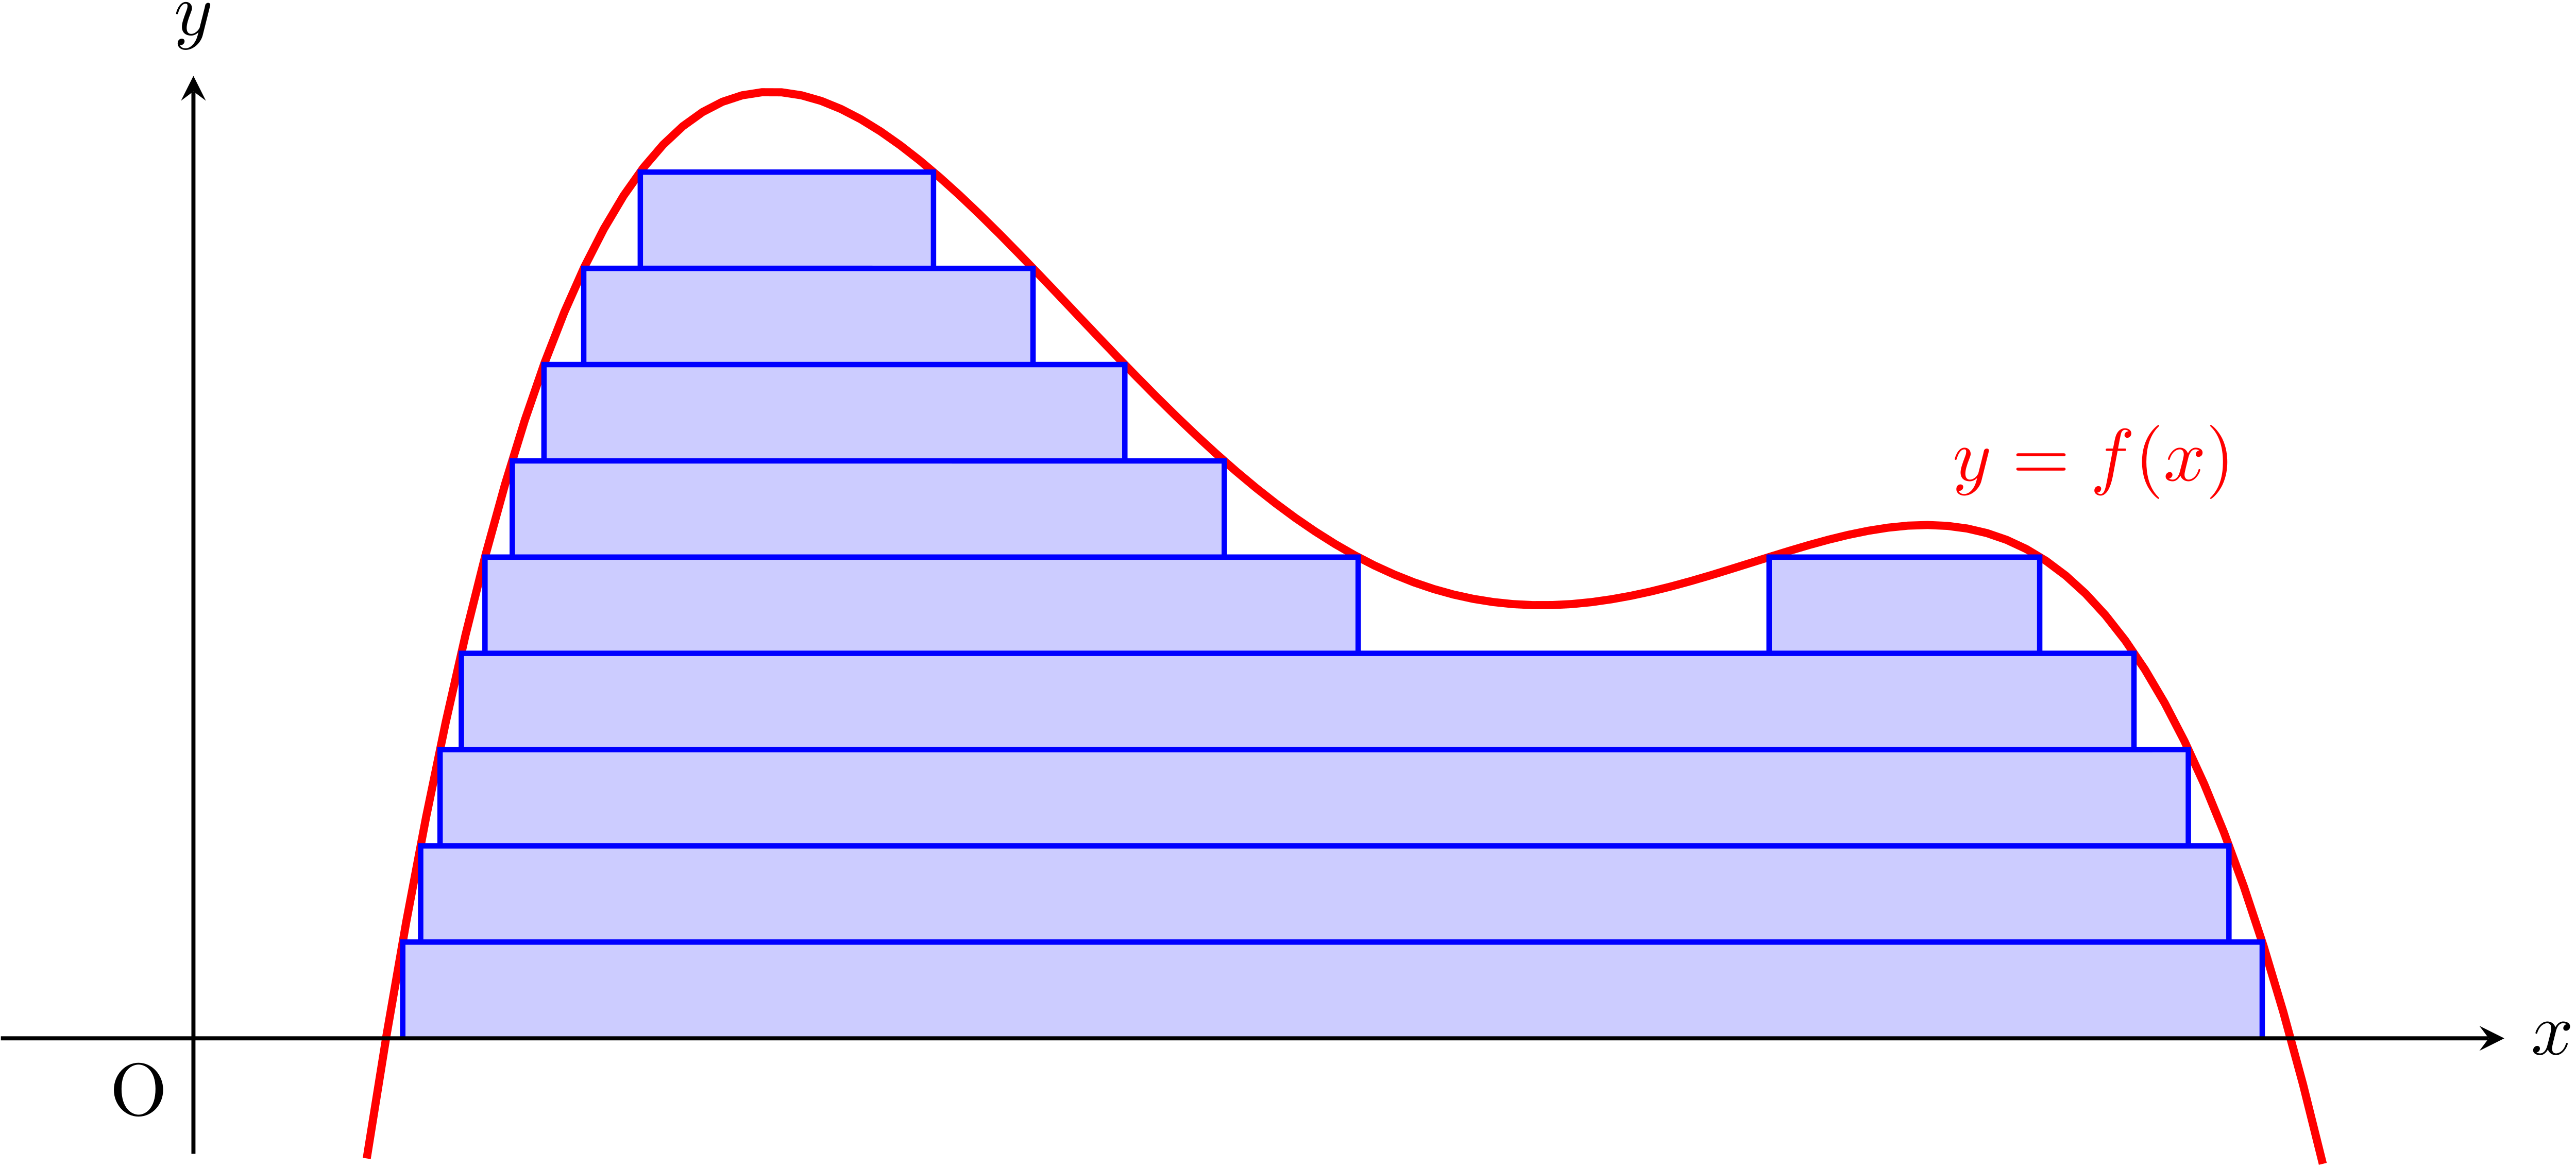
\includegraphics[scale=0.08]{figure/LI}
	\caption{Lebesgue积分示意图}
\end{figure}

\vskip 0.2cm
\begin{theorem}[非负可测简单函数积分的线性性]
	设$\varphi(x),\psi(x)$为$E \subset \R^n$上的非负可测简单函数, 
	$\alpha,\beta$为非负常数, 则有
	\begin{equation}
		\int_E (\alpha \varphi + \beta \psi) \d x = \alpha \int_E \varphi \d x + \beta \int_E \psi \d x.
	\end{equation}
\end{theorem}

\vskip 0.2cm
\begin{theorem}[非负可测简单函数积分的自可列可加性]
	设$\{ E_n \}_{n=1}^{\infty}$为递增可测集列, 
	$\varphi(x)$为$E = \bigcup\limits_{n=1}^{\infty} E_n$上的可测函数, 则
	\begin{equation}
		\lim\limits_{n\to\infty} \int_{E_n} \varphi(x) \d x = \int_E \varphi(x) \d x.
	\end{equation}
\end{theorem}

%%%%%%%%%%%%%%%%%%%%%%%%%%%%%%%%%%%%%%%%%%%%%%%%%%%%%%%%%%%%%%%%%%%%%%%%%%%%%%
%
%										下一小节
%
%%%%%%%%%%%%%%%%%%%%%%%%%%%%%%%%%%%%%%%%%%%%%%%%%%%%%%%%%%%%%%%%%%%%%%%%%%%%%%
\subsection{非负可测函数的Lebesgue积分}

\begin{definition}[非负可测函数的Lebesgue积分]
	设$E \subset \R^n$为可测集, $f(x)$为$E$上的一个非负可测函数, 定义$f(x)$在$E$上的Lebesgue积分为
	\begin{equation}
		\int_E f(x) \d x = \sup\limits_{\varphi \leq f \atop x\in E} 
		\left\{ \int_E \varphi(x) \d x : \varphi(x) \text{为} E \text{上的简单函数} \right\}.
	\end{equation}
	显然$0 \leq \int_E f(x) \d x \leq + \infty$, 
	若$\int_E f(x) \d x < \infty$, 则称$f(x)$在$E$上Lebesgue可积.
\end{definition}

\vskip 0.2cm
\begin{theorem}
	设$f(x),g(x)$为$E \subset \R^n$上的非负可测函数, $A$为$E$的可测子集, 则
	\begin{enumerate}
		\item 若$f \leq g$ a.e.于$E$, 则$\int_E f(x) \d x \leq \int_E g(x) \d x$; 这时若$g(x)$在$E$上可积, 则$f(x)$也在$E$上可积; 
		\item 若$\int_E f(x) \d x = 0$, 则$f(x) = 0$ a.e.于$E$;
		\item 若$\int_E f(x) \d x < \infty$, 则$0 \leq f(x) < \infty$ a.e.于$E$;
		\item $\int_A f(x) \d x = \int_E f(x) \cdot \chi_A \d x \leq \int_E f(x) \d x$. 
	\end{enumerate}
\end{theorem}
\begin{proof}\par 
	1.令$E_1 = E[f \leq g], E_2 = E[f > g]$, 则$E_1, E_2$都是$E$的可测子集, 且有
	$$
		E_1 \cup E_2 = E, \;
		E_1 \cap E_2 = \varnothing, \;
		m E_2 = 0 , 
	$$
	从而有
	$$
		\int_E f \d x = \int_{E_1} f \d x ,\;
		\int_E g \d x = \int_{E_1} g \d x .
	$$
	对于$E_1$上任一满足$\varphi(x) \leq f(x) \leq g(x)$的非负简单函数$\varphi(x)$,
	由定义有$\int_{E_1} \varphi \d x \leq \int_E g \d x = \int_{E_1} g \d x$.
	由此可得
	$$
		\int_{E_1} f(x) \d x = \sup\limits_{\varphi \leq f } 
		\left\{ \int_{E_1} \varphi(x) \d x \right\}
		\leq \int_{E_1} g(x) \d x .
	$$
	从而可知
	$$
		\int_E f(x) \d x \leq \int_E g(x) \d x.
	$$
	
	这时若$g(x)$在$E$上可积, 则
	$$
		\int_E f(x) \d x \leq \int_E g(x) \d x < \infty, 
	$$
	故$f(x)$也在$E$上可积
	\par  
	2. \framebox[\width]{截断法}\;
	对任意正整数$n$, 令
	$$
		\begin{aligned}
			A_n &= E\left[ f \geq \frac{1}{n} \right] ,\\
			\varphi_n(x) &= 
			\begin{cases}
				\frac 1n, & x \in A_n, \\
				0, & x \in E \backslash A_n.
			\end{cases}
		\end{aligned}
	$$
	则
	$$
		0 = \int_E f(x) \d x \geq \int_E \varphi_n(x) \d x = \frac 1n \cdot m A_n \geq 0.
	$$
	故$m A_n = 0, \forall n \in \N^*$. 
	而$E[f>0] = \bigcup\limits_{n=1}^{\infty} A_n$. 
	故$m E[f>0] = 0$, 因而$f(x) = 0$ a.e.于$E$.
	\par 
	3. \framebox[\width]{截断法}\;
	令$E_{\infty} = E[f = +\infty]$. 
	对任意正整数$n$, 令
	$$
		\varphi_n(x) = 
		\begin{cases}
			n, & x\in E_{\infty}, \\
			0, & x\in E \backslash E_{\infty}.
		\end{cases}
	$$
	则
	$$
		\infty > \int_E f(x) \d x \geq \int_E \varphi_n(x) \d x = n \cdot m E_{\infty} \geq 0.
	$$
	故
	$$
		0 \leq m E_{\infty} \leq \frac 1n \int_E f(x) \d x, \; \forall n \in \N^*.
	$$
	所以$m E_{\infty} = 0$, 即有$0 \leq f(x) < \infty$ a.e.于$E$
\end{proof}

\vskip 0.2cm
\begin{theorem}[Levi非负渐升列积分定理] \label{thm:Levi}
	设有定义在可测集$E \in \R^n$上的非负可测函数渐升列
	$$
		f_1(x) \leq f_2(x) \leq \cdots \leq f_k(x) \leq \cdots,
	$$
	令$f(x) = \lim\limits_{n \to \infty} f_n(x), x \in E$, 则
	\begin{equation}
		\lim\limits_{n \to \infty} \int_E  f_n(x) \d x = \int_E  f(x) \d x.
	\end{equation}
\end{theorem}
\begin{proof}
	显然有$f(x)$在$E$非负可测且$f_n(x) \leq f_{n+1}(x) \leq f(x)$, 故
	$$
		 \int_E  f_n(x) \d x \leq \int_E  f_{n+1}(x) \d x \leq \int_E  f(x) \d x.
	$$
	因而
	$$
		\lim\limits_{n \to \infty} \int_E  f_n(x) \d x \leq \int_E  f(x) \d x.
	$$
	下证相反的不等式. \par 
	任取$0<c<1$, 
	$\varphi(x)$为$E$上一简单非负函数, 满足$0 \leq \varphi(x) \leq f(x), \forall x \in E$. 
	记$E_n = E[f_n(x) \geq c\varphi] \subset E$, 显然有$E_n \subset E_{n+1}$, 
	且$\lim\limits_{n \to \infty} E_n = \bigcup\limits_{n=1}^{\infty} E_n = E$, 于是有不等式
	$$
		\int_E f_n(x) \d x \geq \int_{E_n} f_n(x) \d x \geq \int_{E_n} c \varphi(x) \d x = c\int_{E_n} \varphi(x) \d x.
	$$
	根据非负简单函数积分的自可列可加性, 可知
	$$
		\lim\limits_{n \to \infty} \int_{E_n} \varphi(x) \d x = \int_E \varphi(x) \d x .
	$$
	综上我们得到
	$$
		\lim\limits_{n \to \infty} \int_E f_n(x) \d x \geq c \int_E \varphi(x) \d x .
	$$
	上式中令$c \to 1$, 有
	$$
		\lim\limits_{n \to \infty} \int_E f_n(x) \d x \geq \int_E \varphi(x) \d x .
	$$
	再由非负可测函数积分的定义, 有
	$$
		\lim\limits_{n \to \infty} \int_E  f_n(x) \d x \geq \int_E  f(x) \d x.
	$$
\end{proof}

上述定理表明, 对于非负可测函数渐升列来说, 极限与积分的次序可以交换. 
此外, 由于非负可测函数是非负可测简单函数渐升列的极限, 因而使得积分理论中的许多结果可直接从可测简单函数的积分性质得到. 

\vskip 0.2cm
\begin{theorem}[非负可测函数积分的线性性]
	设$f(x),g(x)$为$E \subset \R^n$上的非负可测函数, 
	$\alpha,\beta$为非负常数, 则有
	\begin{equation}
		 \int_E (\alpha f + \beta g) \d x = \alpha \int_E f \d x + \beta \int_E g \d x.
	\end{equation}
\end{theorem}

\vskip 0.2cm
\begin{theorem}[逐项积分定理]
\label{thm:Progressive Integral}
	设$\{ f_n (x) \}$是E上的非负可测函数列, 则
	\begin{equation}
		\int_E \left( \sum\limits_{n = 1}^{\infty} f_n(x) \right) \d x
		= \sum\limits_{n = 1}^{\infty} \int_E f_n(x) \d x.
	\end{equation}
\end{theorem}
\begin{proof}
	令$S_n (x) = \sum\limits_{k = 1}^{n} f_k(x)$, 
	则$\{ S_n(x) \}$为$E$上非负可测函数渐升列. 
	从而根据Levi非负渐升列积分定理(Thm:\ref{thm:Levi})以及积分的线性性质, 可知
	$$
	\begin{aligned}
		\int_E \left( \sum\limits_{n = 1}^{\infty} f_n(x) \right) \d x
		& = \int_E \left(\lim\limits_{n \to \infty} S_n(x)  \right) \d x 
		 = \lim\limits_{n \to \infty} \int_E S_n(x) \d x \\
		& = \lim\limits_{n \to \infty} \sum\limits_{k = 1}^{n} \int_E f_n(x) \d x
		 = \sum\limits_{n = 1}^{\infty} \int_E f_n(x) \d x.
	\end{aligned}
	$$
\end{proof}

\vskip 0.2cm
\begin{theorem}[Fatou引理]
	设$\{ f_n (x) \}$是$E$上的非负可测函数列, 则
	\begin{equation}
		\int_E \varliminf\limits_{n \to \infty} f_n(x) \d x \leq 
		\varliminf\limits_{n \to \infty} \int_E f_n(x) \d x .
	\end{equation}
\end{theorem}
\begin{proof}
	令$g_n (x) = \inf \{ f_k(x) : k \geq n \}$, 
	则$\{ g_n(x) \}$为$E$上的非负可测渐升函数列, 且$x \in E$时有
	$$
		0 \leq g_n(x) \leq g_{n+1}(x) \leq f_{n+1}(x).
	$$
	从而由Levi非负渐升列积分定理(Thm:\ref{thm:Levi})
	$$
		\int_E \varliminf\limits_{n \to \infty} f_n(x) \d x
		= \int_E \lim\limits_{n \to \infty} g_n(x) \d x
		= \lim\limits_{n \to \infty} \int_E g_n(x) \d x
		\leq \varliminf\limits_{n \to \infty} \int_E f_n(x) \d x .
	$$
\end{proof}
\vskip 0.4cm
Fatou引理常用于判断极限函数的可积性. 
例如, 当$E$上的非负可测函数列$\{ f_n (x) \}$满足
$$
	\int_E f_k(x) \d x \leq M \quad k=1,2,\cdots
$$
时, 我们就得到
$$
	\int_E \varliminf\limits_{n \to \infty} f_n(x) \d x \leq M .
$$

下面的例子说明Fatou引理中的不等号是可能成立的. 

\begin{example}
	在$[0,1]$上作非负可测函数列
	$$
	f_n(x) = 
	\begin{cases}
		0, & x=0, \\
		n, & 0 < x < \frac{1}{n}, \\
		0, & \frac{1}{n} < x <1,
	\end{cases}
	\quad n = 1,2,\cdots
	$$
	显然有$\lim\limits_{n \to \infty} f_n(x) = 0 \;(x \in [0,1]).$
	因此
	$$
		\int_{[0,1]} \varliminf\limits_{n \to \infty} f_n(x) \d x = 0 
		< 
		1 = \varliminf\limits_{n \to \infty} \int_{[0,1]} f_n(x) \d x .
	$$
\end{example}




%%%%%%%%%%%%%%%%%%%%%%%%%%%%%%%%%%%%%%%%%%%%%%%%%%%%%%%%%%%%%%%%%%%%%%%%%%%%%%
%
%										下一小节
%
%%%%%%%%%%%%%%%%%%%%%%%%%%%%%%%%%%%%%%%%%%%%%%%%%%%%%%%%%%%%%%%%%%%%%%%%%%%%%%
\subsection{一般可测函数的Lebesgue积分}

\begin{definition}[一般可测函数的Lebesgue积分]
	设$f(x)$为$E \subset \R^n$上的可测函数, 若积分
	$$
		\int_E f^+ (x) \d x, \;
		\int_E f^- (x) \d x
	$$
	中至少有一个是有限值, 则称$f$在$E$上的\textbf{积分确定}, 称
	$$
		\int_E f (x) \d x = \int_E f^+ (x) \d x - \int_E f^- (x) \d x
	$$
	为$f$在$E$上的\textbf{Lebesgue积分}; 
	当上式右端两个积分值皆为有限时, 则称$f$在$E$上是\textbf{可积}的. 
	在$E$上可积的函数的全体记为$L(E)$.
\end{definition}

由于$\int_E |f (x)| \d x = \int_E f^+ (x) \d x + \int_E f^- (x) \d x$, 
故知在$f$可测的条件下, $f(x)$的可积性与$| f(x) |$的可积性是等价的. 
此时还有$|\int_E f \d x| \leq \int_E |f| \d x$. 


\begin{theorem}[$L$积分的一些基本性质]
	\begin{enumerate}
		\item (零测集上实函数$L$可积) \\
		\quad  若$E \neq \varnothing$但$mE=0$, 则$E$上的任何实函数$f$都在$E$上$L$可积且
			$$
				\int_E f \d x = 0;
			$$
		\vskip 0.2cm
		\item ($L$可积函数几乎处处有限) \\
		\quad  若$f \in L(E)$, 则$m E[|f| = \infty] = 0$, 即$|f(x)| < \infty$ a.e.于$E$; 
		\vskip 0.2cm
		\item ($L$积分定义域具有可加性) \\
		\quad 设$f$在可测集$A,B$上积分确定, 且$A \cap B = \varnothing$, 那么
		$$
			\int_{A \cup B} f(x) \d x = \int_{A} f(x) \d x+\int_{B} f(x) \d x ;
		$$
		\vskip 0.2cm
		\item (a.e.相等的函数的$L$积分a.e.相等) \\
		\quad 设$f$在$E$上积分确定, 且$f(x)=g(x)$ a.e.于$E$, 那么$g$也在$E$上积分确定且
		$$
			\int_{E} f(x) \d x = \int_{E} g(x) \d x .
		$$
		特别的, 若$mE < \infty$且$b \leq f(x) \leq B$ a.e.于E, 则
		$$
			bmE \leq \int_E f(x) \d x \leq BmE;
		$$
		\vskip 0.2cm
		\item ($L$积分的保序性) \\
		\quad 设$f, g$在$E$上积分确定, 且$f(x) \leq g(x)$ a.e.于$E$, 那么
		$$
			\int_{E} f(x) \d x \leq \int_{E} g(x) \d x ;
		$$
		\vskip 0.2cm
		\item ($L$积分的绝对值小于等于绝对值的$L$积分)\\
		\quad 设$f$在$E$上$L$可积, 则$|f|$在$E$上亦$L$可积, 且
		$$
			\left|\int_{E} f(x) \d x \right| \leq \int_{E} |f(x)| \d x ;
		$$
		\vskip 0.2cm
		\item (控制可积) \\
		\quad 设$f$在$E$上可测, $g$是$E$上的非负$L$可积函数且$|f(x)| \leq g(x)$ a.e.于$E$, 则$f$在$E$上$L$可积且
		$$
			\left|\int_{E} f(x) \d x \right| \leq \int_{E} |f(x)| \d x \leq \int_{E} g(x) \d x. 
		$$
		一般我们称$g(x)$为$f(x)$的控制函数. 
	\end{enumerate}
\end{theorem}

\vskip 0.2cm
\begin{theorem}[$L$积分的线性性]
	设$f(x),g(x)$为$E \subset \R^n$上的$L$可积函数, 
	对任意$\alpha,\beta \in \R$, 有
	\begin{equation}
		 \int_E (\alpha f + \beta g) \d x = \alpha \int_E f \d x + \beta \int_E g \d x.
	\end{equation}
\end{theorem}

\vskip 0.2cm
\begin{theorem}[$L$积分的绝对连续性]
	设$f$为$E$上可积函数, 则对任意$\varepsilon > 0$, 存在$\delta > 0$, 
	使得对于任意$E$的可测子集$A$满足$mA < \delta$时, 有
	\begin{equation}
		\left| \int_A f(x) \d x \right| \leq \int_A |f(x)| \d x < \varepsilon.
	\end{equation}
\end{theorem}
\begin{proof}
	由于$f \in L(E)$, 故$|f(x)| \in L(E)$. 
	由Riesz表示定理(Thm:\ref{thm:Riesz1}), 对于任意$\varepsilon > 0$, 
	存在$E$上的简单函数满足$0 \leq \varphi(x) \leq |f(x)|$, 且
	$$
		\int_E |f(x)| \d x - \frac{\varepsilon}{2} 
		\leq \int_E \varphi(x) \d x
		\leq \int_E |f(x)| \d x.
	$$
	令$M = \max \{ \varphi(x): x \in E \}$, 
	$\delta = \frac{\varepsilon}{1 + 2M}$, 
	则对于任何可测集$A \subset E$, 只要有$mA < \delta$, 就有
	$$
	\begin{aligned}
		\left| \int_A f(x) \d x \right| 
		&\leq \int_A |f(x)| \d x \\
		&= \int_A (|f(x)| - \varphi(x)) \d x + \int_A \varphi(x) \d x \\
		&\leq \frac{\varepsilon}{2} + M \cdot mA \\
		&< \frac{\varepsilon}{2} + M \cdot \frac{\varepsilon}{1 + 2M} 
		< \varepsilon. 
	\end{aligned}
	$$
\end{proof}

\begin{theorem}[$L$积分对定义域的可数可加性]
	设可测子集列$\{ E_n \}$满足$E_i \cap E_j = \varnothing \; (i \neq j)$. 
	$f$在$E = \bigcup\limits_{n = 1}^{\infty} E_n$上积分确定, 则
	\begin{equation}
		\int_E f(x) \d x = \sum\limits_{n = 1}^{\infty} \int_{E_n} f(x) \d x.
	\end{equation}
\end{theorem}
\begin{proof}
	对任意$n \in \N^*$, 
	令$f_n = f^+ \cdot \chi_{E_n}, g_n = f^- \cdot \chi_{E_n}$, 则
	$$
		f^+(x) = \sum\limits_{n = 1}^{\infty} f_n(x) , \;
		f^-(x) = \sum\limits_{n = 1}^{\infty} g_n(x) . 
	$$
	由逐项积分定理(Thm:\ref{thm:Progressive Integral})
	$$
	\begin{aligned}
		\int_E f(x) \d x
		&= \int_E f^+(x) \d x - \int_E f^-(x) \d x \\
		&= \int_E \sum\limits_{n = 1}^{\infty} f_n(x) \d x 
			- \int_E \sum\limits_{n = 1}^{\infty} g_n(x) \d x \\
		&= \sum\limits_{n = 1}^{\infty} \int_{E_n} f^+(x) \chi_{E_n} \d x
			- \sum\limits_{n = 1}^{\infty} \int_{E_n} f^-(x) \chi_{E_n} \d x \\
		&= \sum\limits_{n = 1}^{\infty} \int_{E_n} f^+(x) \d x
			- \sum\limits_{n = 1}^{\infty} \int_{E_n} f^-(x) \d x \\
		&= \sum\limits_{n = 1}^{\infty} \int_{E_n} (f^+(x) - f^-(x)) \d x
	\end{aligned}
	$$
\end{proof}



\begin{theorem}[积分变量的平移变换定理]
	若$f \in L( E )$, 则对任意的$x_0 \in E, \; f(x+x_0) \in L( E )$, 有
	\begin{equation}
		\int_E f(x + x_0) \d x = \int_E f(x) \d x.
	\end{equation}
\end{theorem}
\begin{proof}
	只需考虑$f \geq 0$的情形. 
	首先考虑$f$为非负可测简单函数:
	$$
		f(x) = \sum\limits_{i=1}^n c_i \chi_{E_i}(x) , \; x\in E. 
	$$
	显然有
	$$
		f(x + x_0) = \sum\limits_{i=1}^n c_i \chi_{E_i - \{x_0\}}(x) , \; x\in E
	$$
	仍为非负可测简单函数,从而
	$$
	\begin{aligned}
		\int_E f(x + y_0) \d x &= 
		\sum\limits_{i=1}^n c_i m( E_i - \{x_0\} ) \\
		&= \sum\limits_{i=1}^n c_i m( E_i ) = \int_E f(x) \d x.
	\end{aligned}
	$$
	
	其次, 考虑一般非负可测函数$f(X)$. 
	此时存在非负可测简单函数渐升列$\{ \varphi_n (x) \}$, 使得$\lim\limits_{n \to \infty} \varphi_n (x) = f(x), \; x \in E$. 
	显然$\{ \varphi_n (x + x_0) \}$仍为渐升列, 且有
	$$
		\lim\limits_{n \to \infty} \varphi_n (x + x_0) = f(x + x_0), \; x \in E.
	$$
	从而
	$$
	\begin{aligned}
		\int_E f(x + y_0) \d x &= 
		\lim\limits_{n \to \infty} \int_E \varphi_n (x + y_0) \d x \\
		&= \lim\limits_{n \to \infty} \int_E \varphi_n (x)\d x = \int_E f(x) \d x.
	\end{aligned}
	$$
\end{proof}

\begin{definition}[平均收敛]
	设$\{ f_n(x) \}$为$E$上的可积函数列, $f(x)$在$E$上可积, 若
	$$
		\lim\limits_{n \to \infty} \int_E |f_n -f| \d x = 0,
	$$
	则称$\{ f_n(x) \}$(1次幂)\textbf{平均收敛}于$f(x)$.
\end{definition}

\begin{theorem}[平均收敛一定依测度收敛]
	设$\{ f_n(x) \}$为$E$上的可积函数列, $f(x)$在$E$上可积, 若
	$$
		\lim\limits_{n \to \infty} \int_E |f_n -f| \d x = 0,
	$$
	那么有$\{ f_n(x) \}$依测度收敛于$f(x)$. 
\end{theorem}

\begin{proof}
	\framebox[\width]{截断法}\;
	对任意$\sigma > 0$, 记$E_n = E[|f_n - f| \geq \sigma]$, 由
	$$
	\begin{aligned}
		\sigma m E_n 
		&= \int_{E_n} \sigma \d x 
		\leq \int_{E_n} |f_n - f| \d x \\
		&\leq \int_E |f_n - f| \d x \to 0 \quad (n \to \infty)
	\end{aligned}
	$$
	所以有$\lim\limits_{n \to \infty} m E_n = 0$. 
\end{proof}

进一步地, 由Riesz定理(Thm:\ref{thm:Riesz2}), 存在子列$\{ f_{n_j}(x) \}$使得
$$
	\lim\limits_{j \to \infty} f_{n_j}(x) = f(x) \quad \text{a.e.} x \in E.
$$

\begin{proposition}[闭区间上存在连续函数平均收敛于$L$可积函数]
	设$f \in L[a,b]$, 则对于任意$\varepsilon >0$, 存在$g \in C[a,b]$, 使得
	$$
		\int_{[a,b]} |f(x) - g(x)| < \varepsilon.
	$$
\end{proposition}
\begin{proof}  
\framebox[\width]{简单函数$\varphi(x)$逼近$f(x)$} \par 
由于$f \in L[a, b]$, 故$f^+$和$f^-$都在$[a, b]$上非负$L$可积.
对于任意的$\varepsilon>0$, 存在$[a, b]$上的两个非负简单函数$\varphi_{1}$和$\varphi_{2}$, 
使得$x \in[a, b]$时, $0 \leq \varphi_1 (x) \leq f^+(x), 0 \leq \varphi_2 (x) \leq f^-(x)$. 且
$$
\begin{array}{l}
\int_{[a, b]} f^+(x) \d x-\frac{\varepsilon}{4} \leq \int_{[a, b]} \varphi_1 (x) \d x \leq \int_{[a, b]} f^+(x) \d x \\
\int_{[a, b]} f^-(x) \d x-\frac{\varepsilon}{4} \leq \int_{[a, b]} \varphi_2 (x) \d x \leq \int_{[a, b]} f^-(x) \d x
\end{array}
$$
令$\varphi(x)=\varphi_1 (x)-\varphi_2 (x)$, 
则$\varphi$是$[a, b]$上的简单函数, 且
$$
\begin{aligned}
\int_{[a, b]}|f(x)-\varphi(x)| \d x &=\int_{[a, b]}\left|f^+(x)-f^-(x)-\varphi_1 (x)+\varphi_2 (x)\right| \d x \\
& \leq \int_{[a, b]}\left|f^+(x)-\varphi_1 (x)\right| \d x+\int_{[a, b]}\left|f^-(x)-\varphi_2 (x)\right| \d x \\
&=\left(\int_{[a, b]} f^+(x) \d x-\int_{[a, b]} \varphi_1 (x) \d x\right)+\left(\int_{[a, b]} f^-(x) \d x-\int_{[a, b]} \varphi_2 (x) \d x\right) \\
& \leq \frac{\varepsilon}{4}+\frac{\varepsilon}{4}=\frac{\varepsilon}{2}.
\end{aligned}
$$ 

\framebox[\width]{根据Лузин定理', 此处直接写出$g$存在性即可} \par
令 $M=\max \{|\varphi(x)|: x \in[a, b]\}$, 
令 $\delta=\frac{\varepsilon}{1+4 M}$, 
由Лузин定理'(Thm:\ref{thm:Lusin2}), 
存在闭集$F \subset[a, b]$满足$m([a, b] \backslash F)<\delta$
以及$g \in C[a, b]$, 使得对任意$x \in F$, 有$g(x)=\varphi(x)$; 
且$x \in[a, b]$时, 有$|g(x)| \leq M$. 
于是
$$
\begin{aligned}
	\int_{[a, b]}|\varphi(x)-g(x)| \d x
	&= \int_{[a, b] \backslash F}|\varphi(x)-g(x)| \d x \\
	&\leq \int_{[a, b] \backslash F}|\varphi(x)| \d x - \int_{[a, b] \backslash F}|g(x)| \d x \\
	&< M \delta + M \delta < \frac{\varepsilon}{2}.
\end{aligned}
$$
因而
$$
\begin{aligned}
	     & \int_{[a,b]} |f(x) - g(x)| \d x \\
	\leq & \int_{[a, b]}|f(x)-\varphi(x)| \d x + \int_{[a, b]}|\varphi(x)-g(x)| \d x \\
	<    & \frac{\varepsilon}{2} + \frac{\varepsilon}{2} = \varepsilon.
\end{aligned}
$$
\end{proof}


































%%%%%%%%%%%%%%%%%%%%%%%%%%%%%%%%%%%%%%%%%%%%%%%%%%%%%%%%%%%%%%%%%%%%%%%%%%%%%%
%
%										下一节
%
%%%%%%%%%%%%%%%%%%%%%%%%%%%%%%%%%%%%%%%%%%%%%%%%%%%%%%%%%%%%%%%%%%%%%%%%%%%%%%
\section{积分收敛定理}

控制收敛定理的直接结论是平均收敛, 为积分与极限次序的交换所提供的了充分条件. 
它是Lebesgue积分理论中最重要的结果之一.

\begin{theorem}[Lebesgue控制收敛定理]\label{thm:Ldc}
	设$\{ f_n(x) \}_{n=1}^{\infty}$为$E$上的可测函数列, 且有
	$$
		\lim\limits_{n \to \infty} f_n(x) = f(x), \; a.e. x \in E.
	$$
	若存在$E$上的可积函数$F(x)$, 使得对任意的$n \in \N^*$
	$$
		|f_n(x)| \leq F(x), \; a.e. x \in E ,
	$$
	则
	\begin{enumerate}
		\item 
		\begin{equation}
			\lim\limits_{n\to\infty}\int_E |f_n(x) - f(x)| \d x = 0,
		\end{equation}
		
		\item 
		\begin{equation}
			\lim\limits_{n\to\infty}\int_E f_n(x) \d x = \int_E f(x)\d x.
		\end{equation}
	\end{enumerate}
	
	(通常称$F(x)$为函数列$\{ f_n(x) \}$的\textbf{控制函数}.)
\end{theorem}
\begin{proof} 
	\framebox[\width]{记$g_n(x) = |f_n(x) - f(x)|$} \par 
	显然$f$在$E$上可测且$|f(x)| \leq F(x) \;\text{a.e.} x\in E$. 
	从而$f(x)$, 每个$f_n(x)$均可积. 
	
	令$g_n(x) = |f_n(x) - f(x)|$, 则$g(x)$在$E$上可积且满足
	$$
	\begin{aligned}
		& 0 \leq g_n(x) \leq |f_n(x)| + |f(x)| \leq 2F(x), \\ 
		& \lim\limits_{n \to \infty} g_n(x) = 0, 
	\end{aligned}
		 \quad a.e. x \in E.
	$$
	从而有
	$$
	\begin{aligned}
		& 2F(x) - g_n(x) \geq 0, \\ 
		& \lim\limits_{n \to \infty} 2F(x) - g_n(x) = 2F(x), 
	\end{aligned}
		 \quad a.e. x \in E.
	$$
	\framebox[\width]{由Fatou引理"压平"$g_n(x)$} \par
	由Fatou引理
	$$
	\begin{aligned}
		2 \int_E F(x) \d x
		&= \int_E \lim\limits_{n \to \infty} (2F(x) - g_n(x)) \d x \\
		&\leq \varliminf\limits_{n \to \infty} \int_E (2F(x) - g_n(x)) \d x \\
		&= 2 \int_E F(x) \d x + \varliminf\limits_{n \to \infty} \left(- \int_E g_n(x) \d x \right) \\
		&= 2 \int_E F(x) \d x - \varlimsup\limits_{n \to \infty} \int_E g_n(x) \d x.
	\end{aligned}
	$$
	故$\varlimsup\limits_{n \to \infty} \int_E g_n(x) \d x \leq 0$,
	又$\int_E g_n(x) \d x \geq 0$, 
	从而$\lim\limits_{n \to \infty} \int_E g_n(x) \d x = 0$, 
	即
	$$
		\lim\limits_{n \to \infty} \int_E |f_n(x) - f(x)| \d x = 0.
	$$
	从而
	$$
		0 \leq 
		\lim\limits_{n \to \infty} \left| \int_E f_n(x) \d x - \int_E f(x) \d x \right|
		\leq \lim\limits_{n \to \infty} \int_E |f_n(x) - f(x)| \d x = 0
	$$
\end{proof}

\begin{theorem}[依测度收敛型Lebesgue控制收敛定理]
	设$\{ f_n(x) \}_{n=1}^{\infty}$为$E$上的可测函数列, 
	且$f_n(x)$在$E$上依测度收敛于$f(x)$. 
	若存在$E$上的可积函数$F(x)$, 使得对任意的$n \in \N^*$
	$$
		|f_n(x)| \leq F(x), \; a.e. x \in E ,
	$$
	则
	\begin{enumerate}
		\item 
		\begin{equation}
			\lim\limits_{n\to\infty}\int_E |f_n(x) - f(x)| \d x = 0,
		\end{equation}
		
		\item 
		\begin{equation}
			\lim\limits_{n\to\infty}\int_E f_n(x) \d x = \int_E f(x)\d x.
		\end{equation}
	\end{enumerate}
\end{theorem}
\begin{proof}
	反证法. 
	设有$\lim\limits_{n \to \infty}\int_E |f_n(x) - f(x)| \d x \neq 0$, 
	则存在$\{ f_n \}$的子列$\{ f_{n_j} \}$使得
	$$
	\begin{array}{c r}
		\lim\limits_{j\to\infty}\int_E |f_{n_j}(x) - f(x)| \d x = \alpha >0. 
		&  (*)
	\end{array}
	$$
	又$\{ f_{n_j} \}$依测度收敛于$f(x)$, 根据Riesz定理(Thm:\ref{thm:Riesz2}), 
	存在$\{ f_{n_j} \}$的子列$\{ f_{n_{j_k}} \}$使得
	$$
		\lim\limits_{k\to\infty}  f_{n_{j_k}}(x) = f(x),\;\text{a.e.} x\in E.
	$$
	由Lebesgue控制收敛定理(Thm:\ref{thm:Ldc}), 
	$$
		\lim\limits_{k\to\infty}\int_E |f_{n_{j_k}}(x) - f(x)| \d x = 0.
	$$
	这与($*$)式相矛盾, 故
	$$
		\lim\limits_{n\to\infty}\int_E |f_n(x) - f(x)| \d x = 0.
	$$
\end{proof}

\begin{corollary}
	设$E \subset \R^n$为可测集, $m E < \infty$, $f$和$f_n\;(n=1,2,\cdots)$都是$E$上的可测函数. 
	如果存在$M > 0$使得对于任意的正整数$n$, $| f_n | \leq M$ a.e.$x \in E$, 且$n \to \infty$时有
	$$
		f_n(x) \to f(x) \;\text{a.e.} x \in E
		\text{或}
		f_n(x) \text{依测度收敛于} f, 
	$$
	则
	\begin{enumerate}
		\item 
		\begin{equation}
			\lim\limits_{n\to\infty}\int_E |f_n(x) - f(x)| \d x = 0,
		\end{equation}
		
		\item 
		\begin{equation}
			\lim\limits_{n\to\infty}\int_E f_n(x) \d x = \int_E f(x)\d x.
		\end{equation}
	\end{enumerate}	
\end{corollary}

\begin{theorem}[逐项积分定理]
	设$\{ f_n(x) \}_{n=1}^{\infty}$为$E$上的$L$可积函数列, 如果正项级数$\sum\limits_{n = 1}^{\infty} \int_E | f_n(x) | \d x$收敛, 则函数项级数$\sum\limits_{n = 1}^{\infty} f_n(x)$在$E$上a.e.收敛, 其和函数在$E$上$L$可积且
	\begin{equation}
		\int_E \sum\limits_{n = 1}^{\infty} f_n(x) \d x =
		\sum\limits_{n = 1}^{\infty} \int_E f_n(x) \d x.
	\end{equation}
\end{theorem}
\begin{proof}
	令
	$$
		F(x) = \sum\limits_{n = 1}^{\infty} |f_n(x)|, \; x \in E.
	$$
	由逐项积分定理(Thm:\ref{thm:Progressive Integral})
	$$
		\int_E F(x) \d x
		= \int_E \sum\limits_{n = 1}^{\infty} |f_n(x)| \d x
		= \sum\limits_{n = 1}^{\infty} \int_E |f_n(x)| \d x
		< \infty.
	$$
	故$F(x)$在$E$上非负$L$可积, 所以$0 \leq F(x) < \infty$ a.e.$x \in E$, 
	因而$\sum\limits_{n = 1}^{\infty} f_n(x)$在$E$上 a.e.收敛. 
	
	令
	$$
		g(x) = \sum\limits_{n = 1}^{\infty} f_n(x) ,\quad
		g_n(x) = \sum\limits_{k = 1}^{n} f_k(x) ,\quad
		x \in E ,
	$$
	则
	$$
		| g_n(x) | \leq \sum\limits_{k = 1}^{n} | f_k(x) | \leq F(x) 
		\;\text{a.e.} x \in E
	$$
	且$n \to \infty$时, $g_n(x) \to g(x)$ a.e.于$E$, 
	由Lebesgue控制收敛定理(Thm:\ref{thm:Ldc}), $g$在$E$上$L$可积且
	$$
		\begin{aligned}
			\int_E g(x) \d x
			&= \lim\limits_{n \to \infty} \int_E g_n(x) \d x \\
			&= \lim\limits_{n \to \infty} \int_E \sum\limits_{k = 1}^{n} f_k(x) \d x 
			= \lim\limits_{n \to \infty}  \sum\limits_{k = 1}^{n} \int_E f_k(x) \d x \\
			&= \sum\limits_{n = 1}^{\infty} \int_E f_n(x) \d x \; ,
		\end{aligned}
	$$
	即
	$$
		\int_E \sum\limits_{n = 1}^{\infty} f_n(x) \d x =
		\sum\limits_{n = 1}^{\infty} \int_E f_n(x) \d x.
	$$
\end{proof}

\begin{theorem}[积分号下求导]
	设$E \subset \R^n$为可测集, $f(x, t)$为$E \times (a, b)$上的实函数. 
	如果对任意$t_0 \in (a, b)$, $f(x, t_0)$在$E$上$L$可积; 
	对于 a.e.的$x_0 \in E$, $f(x.t)$作为$t$的函数在$(a, b)$上可导且存在
	$\left| \frac{\partial}{\partial t} f(x, t) \right| \leq F(x_0)$, 
	此处的$F$为$E$上某个非负$L$可积函数, 则$\int_E f(x,t) \d x$在$(a,b)$上可导且
	\begin{equation}
		\frac{\d}{\d t} \int_E f(x, t) \d x = \int_E \frac{\partial}{\partial t} f(x, t) \d x.
	\end{equation}
\end{theorem}
\begin{proof}
	任意取定$t \in (a, b)$以及$h_n \to 0 \; (n \to \infty)$, 我们有
	$$
		\lim\limits_{n \to \infty} \frac{f(x, t+h_n) - f(x, t)}{h_n}
		= \frac{\partial}{\partial t} f(x, t), \; x\in E.
	$$
	且当$k$充分大时, 由微分中值定理, 有下式成立
	$$
		\left| \frac{f(x, t+h_n) - f(x, t)}{h_n} \right|
		= \left| \frac{\partial}{\partial t} f(x, t + \theta_n h_n ) \right|
		\leq F(x) \; \text{a.e.} \; x\in E,
	$$
	其中$0 < \theta_n <1$, 从而由Lebesgue控制收敛定理(Thm:\ref{thm:Ldc})可得
	$$
		\frac{\d}{\d t} \int_E f(x, t) \d x
		= \lim\limits_{n \to \infty} \frac{1}{h_n} \int_E [ f(x, t+h_n) - f(x, t) ] \d x
		= \int_E \lim\limits_{n \to \infty} \frac{f(x, t+h_n) - f(x, t)}{h_n} \d x
		= \int_E \frac{\partial}{\partial t} f(x, t) \d x.
	$$
\end{proof}
%\begin{center}
%\begin{tikzpicture}
%
%	\tikzstyle{every node}=[font=\small,scale=1] %放大
%
%	\node[draw, rounded corners]                       (LC1)   {Lebesgue控制收敛定理};
%	\node[draw, rounded corners, right = 20pt of LC1]  (LC2)  {依测度收敛型Lebesgue控制收敛定理};
%	\node[draw, rounded corners, right = 20pt of LC2] (Levi)   {Levi 非负渐升列积分定理};
%	
%	\tikzstyle{arrow1} = [thick,<->,>=stealth]
%	\draw[arrow1] (LC1)       --    (LC2);
%	\tikzstyle{arrow2} = [thick,->,>=stealth]
%	\draw[arrow2] (LC2)       --    (Levi);
%	
%\end{tikzpicture}	
%\end{center}
%\vskip 0.5cm
%%%%%%%%%%%%%%%%%%%%%%%%%%%%%%%%%%%%%%%%%%%%%%%%%%%%%%%%%%%%%%%%%%%%%%%%%%%%%%
%
%										下一节
%
%%%%%%%%%%%%%%%%%%%%%%%%%%%%%%%%%%%%%%%%%%%%%%%%%%%%%%%%%%%%%%%%%%%%%%%%%%%%%%
\section{Riemann积分与Lebesgue积分}

至此,我们已经基本上建立了Lebesgue积分理论, 在进一步介绍这一理论的其他内容以前, 我们先来揭示它与Riemann积分的关系. 
这一关系可以用一个公式来表达, 它不仅说明Lebesgue积分是Riemann积分的一种推广, 而且为一般有界函数的Riemann可积性提供了一个简明的判别准则. 
本节仅讨论一维的情形.



\begin{theorem}
	设$f(x)$为$[a,b]$上的有界函数, 则$f(x)$在$[a,b]$上$R$可积的充要条件为$f(x)$在$[a,b]$上 a.e.连续, 即$f(x)$的不连续点全体城一零测集. 
\end{theorem}

上述定理指出, 对于$[a,b]$上的有界函数而言, 其$R$可积性并非由函数在不连续点的性态所决定, 而是取决于它的不连续点集的测度. 
下面定理说明了$L$积分是$R$积分的推广.
\begin{theorem}
	设$f(x)$为$[a,b]$上一个有界函数, 若$f(x)$在$[a,b]$上$R$可积, 则$f(x)$在$[a,b]$上$L$可积, 且
	$$
		(L) \int_{[a,b]} f(x) \d x = (R) \int_a^b f(x) \d x.
	$$
\end{theorem}

但是对于无界函数的瑕积分以及无穷区间上的反常积分, 情况就有所不同了, 它原本是一种Cauchy极限意义下的积分思想:
$$
	\int_a^{+\infty} f(x) \d x = \lim\limits_{A \to \infty} \int_a^A f(x) \d x, \quad
	\int_a^b f(x) \d x = \lim\limits_{\varepsilon \to 0^+} \int_a^{b-\varepsilon} f(x) \d x.
$$

$L$积分指的是绝对收敛的积分, 并无条件收敛一说.
下面例子指出一般情况下$L$积分并不是$R$反常积分的推广.
\begin{example}
	令
	$$
		f(x) = 
		\begin{cases}
			\frac{\sin x}{x}, & x>0 , \\
			1, & x=0 .
		\end{cases}
	$$
	则$f(x)$在$[0, +\infty)$上连续, $f(x)$在$[0, +\infty)$上的$R$反常积分收敛
	$$
		(R) \int_0^{+\infty} \frac{\sin x}{x} \d x = \frac{\pi}{2}.
	$$
	但是
	$$
		(L) \int_{[0,+\infty)} f^+(x) \d x
		= \sum\limits_{n=0}^{\infty} (L) \int_{[2n\pi, (2n+1)\pi]} \frac{\sin x}{x} \d x
		\geq \sum\limits_{n=0}^{\infty} (L) \int_{[2n\pi+\frac{\pi}6, 2n\pi+\frac{5\pi}6]} \frac{\sin x}{x} \d x
	$$
	而在区间$[2n\pi+\frac{\pi}6, 2n\pi+\frac{5\pi}6]$上有
	$$
			\sin x \geq \frac{1}{2}, \quad
			\frac{1}{x} \geq \frac{1}{2n\pi+5\pi / 6}. 
	$$
	此时
	$$
		(L) \int_{[0,+\infty)} f^+(x) \d x 
		\geq \sum\limits_{n=0}^{\infty} (L) \int_{[2n\pi+\frac{\pi}6, 2n\pi+\frac{5\pi}6]} \frac{1}{4n\pi+5\pi / 3} \d x
		= \frac{2\pi}{3} \sum\limits_{n=0}^{\infty} \frac{1}{4n\pi+5\pi / 3} 
		= \infty.
	$$
	因此$f(x)$在$[0, +\infty)$上不是积分确定的, 当然不是$L$可积的.
\end{example}

\vskip 0.3cm
特别的, 对\textbf{非负函数}而言$L$积分也是$R$反常积分的推广.  
\begin{theorem}
	设$f(x)$是$[a,\infty)$上一个非负实函数, 若对于任意的$A > a$, $f(x)$在$[a,b]$上$R$可积且$R$反常积分$(R) \int_a^{\infty} f(x) \d x$收敛, 则$f(x)$在$[a,\infty)$上$L$可积且
	$$
		(L) \int_{[a,\infty)} f(x) \d x = (R) \int_a^{\infty} f(x) \d x.
	$$
\end{theorem}



 





%%%%%%%%%%%%%%%%%%%%%%%%%%%%%%%%%%%%%%%%%%%%%%%%%%%%%%%%%%%%%%%%%%%%%%%%%%%%%%
%
%										下一节
%
%%%%%%%%%%%%%%%%%%%%%%%%%%%%%%%%%%%%%%%%%%%%%%%%%%%%%%%%%%%%%%%%%%%%%%%%%%%%%%
\section{重积分与累次积分的关系}

\begin{definition}[直积]
	设$A \subset \R^p, \; B \subset \R^q$为两个非空点集, 则$\R^{p+q}$中的点集$\{ (x,y): x \in A, y \in B \}$称$A$与$B$的\textbf{直积}, 记作$A \times B$.
\end{definition}
\begin{note}
	一般地, $A \times B \neq B \times A$. 
\end{note} 

容易验证, 直积有下列简单性质: 
\begin{enumerate}
	\item 若$A_1 \subset A_2$, 则$A_1 \times B \subset A_2 \times B$; 
	\item 若$A_1 \cap A_2 = \varnothing$, 则$A_1 \times B \cap A_2 \times B = \varnothing$; 
	\item $(\cup_i A_i) \times B = \cup_i (A_i \times B), \; (\cap_i A_i) \times B = \cap_i (A_i \times B)$; 
	\item $(A_1 \backslash A_2) \times B = (A_1 \times B) \backslash (A_2 \times B)$. 
\end{enumerate}

\begin{definition}[截面]
	设$E$为$\R^{p+q}$中一点集, $x_0$为$\R^p$中一个固定点, 则$\R^q$中的点集
	$$
		\{ y \in \R^q: (x_0, y) \in E \}
	$$
	称为$E$关于$x_0$的\textbf{截面}, 记作$E_{x_0}$.
\end{definition}

容易验证, 截面有下列简单性质: 
\begin{enumerate}
	\item 若$A_1 \subset A_2$, 则$(A_1)_x \subset (A_2)_x$; 
	\item 若$A_1 \cap A_2 = \varnothing$, 则$(A_1)_x \cap (A_2)_x = \varnothing$; 
	\item $(\cup_i A_i)_x = \cup_i (A_i)_x, \; (\cap_i A_i)_x = \cap_i (A_i)_x$; 
	\item $(A_1 \backslash A_2)_x = (A_1)_x \backslash (A_2)_x$. 
\end{enumerate}

\vskip 0.4cm
下面定理给了我们一个由低维测度求高维测度的有力工具.

\begin{theorem}[截面定理]\label{thm:cross-section}
	设$E \subset \R^{p+q}$为可测集, 则
	\begin{enumerate}
		\item 对于$\R^p$中的几乎所有点$x$, $E_x$为$\R^q$中的可测集; 
		\item $m E_x$作为$x$的函数, 它是在$\R^p$上a.e.有定义的可测函数;
		\item $m E = \int_{\R^p} m E_x \d x$. 
	\end{enumerate}
\end{theorem}

\vskip 0.2cm
\begin{theorem}
	设$A,B$分别是$\R^p,\R^q$中的可测集, 则$A \times B$是$\R^{p+q}$中的可测集, 且$m (A \times B) = mA \cdot mB$. 	
\end{theorem}

\vskip 0.4cm
\begin{definition}[下方图形]
	设$f(x)$为$E \subset \R^n$中的非负函数, 则$\R^{n+1}$中的点集
	$$
		\{ (x,z): x \in E, 0 \leq z < f(x) \}
	$$
	称为$f(x)$在$E$上的\textbf{下方图形}, 记作$G(E,f)$.
\end{definition}

\vskip 0.2cm
\begin{theorem}[非负可测函数积分的几何意义]\label{thm:Geo-meaning}
	设$f (x)$为可测集$E \subset \R^n$上的非负函数, 则
	\begin{enumerate}
		\item $f(x)$为$E$上可积函数的\textbf{充要条件}为$G(E,f)$为$\R^{n+1}$中的可测集; 
		\item 当$f(x)$在$E$上可测时, 
		$$
			\int_E f(x) \d x = m G(E,f). 
		$$
	\end{enumerate}
\end{theorem}

\vskip 0.2cm
\begin{corollary}
	设$f (x)$为$E$上的可积函数, 则
	$$
		\int_E f(x) \d x = m G(E, f^+) - m G(E,f^-). 
	$$
\end{corollary}

\vskip 0.2cm
\begin{corollary}
	可测函数$f(x)$在$E \in \R^n$上可积的充要条件是$m G(E, f^+)$与$m G(E,f^-)$都有限.
\end{corollary}

\vskip 0.2cm
由上述两个推论立即可以导出 Fubini 定理, 它说明了高维积分与低维积分之间的联系, 也即数学分析中重 积分化为累次积分的推广. 
\begin{theorem}[Fubini-Tonelli定理]\label{thm:Fubini-Tonelli}

\begin{enumerate}
	\item (\textbf{Tonelli, 非负可测函数情形}) 设$f(P) = f(x,y)$在$A \times B \subset \R^{p+q}$($A,B$分别为$\R^p$与$\R^q$中的可测集)上非负可测, 则对a.e. $x \in A$, $f(x,y)$作为$y$的函数在$B$上可测, 且
			\begin{equation}
				\int_{A \times B} f(P) \d P = \int_A \d x \int_B f(x,y) \d y. \label{eq:Fubini}
			\end{equation}	
	\item (\textbf{Fubini, 可积函数情形}) 设$f(P) = f(x,y)$在$A \times B \subset \R^{p+q}$上可积, 则对a.e. $x \in A$, $f(x,y)$作为$y$的函数在$B$上可积, 且$\int_B f(x,y) \d y$作为$x$的函数在$A$上可积且(\ref{eq:Fubini})成立
\end{enumerate}

\end{theorem}

Fubini-Tonelli定理给出了重积分化为累次积分的两个充分条件, 下面我们对该定理给予证明.

\begin{proof}\par
	(1) 由非负可测函数积分的几何意义(thm: \ref{thm:Geo-meaning}), $G(A \times B, f)$为$\R^{p+q+1}$中的可测集, 且
	$$
		m G(A \times B, f) = \int_{A \times B} f(P) \d P, 
	$$
	但是由截面定理(thm: \ref{thm:cross-section}), 可得
	$$
		m G(A \times B, f) = \int_{\R^p} m G(A \times B, f)_x \d x,
	$$
	其中被积函数a.e.有意义. 由于
	$$
		\R^{q+1} \supset G(A \times B, f)_x = 
		\begin{cases}
			\{(y,z): y \in B, 0 \leq z < f(x,y) \}, & x \in A \\
			\varnothing, & x \notin A.
		\end{cases}
	$$
	所以对于$x \in A$, 该截面实际上是将$x$固定后, $f(x,y)$看作是$y$的函数时, 在$B$的下方图形$G(B,f_{(x \text{固定} )})$. 于是当此截面可测时由非负可测函数积分的几何意义有
	$$
		m G(A \times B, f)_x = m G(B, f_{(x \text{固定} )}) = \int_B f(x,y) \d y.
	$$
	结合上式有
	$$
		\int_{A \times B} f(P) \d P = \int_A \d x \int_B f(x,y) \d y.
	$$
	
	(2) 设$f(P)$在$A \times B$上可积, 则$f^+ (P)$, $f^- (P)$在$A \times B$上也可积, 从而有
	$$
	\begin{aligned}
		 \int_{A \times B} f(P) \d P 
		&= \int_{A \times B} f^+(P) \d P - \int_{A \times B} f^-(P) \d P \\
		&= \int_A \d x \int_B f^+(x,y) \d y - \int_A \d x \int_B f^-(x,y) \d y\\
		&= \int_A \d x \left( \int_B f^+(x,y) \d y - \int_B f^-(x,y) \d y \right) \\
		&= \int_A \d x \int_B (f^+(x,y) - f^-(x,y)) \d y  \\
		&= \int_A \d x \int_B f(x,y) \d y. 
	\end{aligned}
	$$
\end{proof}

\begin{note}
	公式(\ref{eq:Fubini})化为
	\begin{equation}
		\int_{A \times B} f(P) \d P = \int_B \d y \int_A f(x,y) \d x
	\end{equation}
	同样成立. 
\end{note}
















